% !TEX root = _main.tex

% ==========================================
% ここから本文．あとは各自で
% ==========================================

%1
\section{はじめに}

近年インターネットの普及に伴い音楽の楽しみ方が大きく変化している．
従来ではCDを購入してプレイヤーで楽しむことが一般的であったが，近年はインターネット配信で楽しむ人が増加している．
各音楽配信サイトなどでは，ユーザの嗜好に合った楽曲の検索を容易にするために楽曲を音楽ジャンル別で分類されることが多くみられる．

しかし，楽曲のジャンルは時系列で変わっていくのではないだろうか？

例として，「Mrs. GREEN APPLE」の「ライラック」\cite{fingofam}があげられる．
この楽曲は，冒頭約10秒間でギターにエフェクトを加えた電子音が流れる．
しかし，その後同じフレーズをドラムやギターの音色で構成する．
これにより，電子音のような音色では感じることのなかったロックミュージックの印象を抱かせるものとなっている．
このように，聴取する箇所によって抱く印象が異なる楽曲が存在すると考える．

また，音楽ジャンル解析は古くから数多くの研究が行われており，近年では主要な研究テーマの１つとして扱われている．
しかし，これらの大半は１つの楽曲を1つの音楽ジャンルに分類するものである．
このような音楽ジャンルの分類方法では，楽曲内における音楽ジャンルの変化の識別が困難であると考える．

そこで本研究では，数ある音響特徴量の中でも音色に着目し，対象楽曲の楽器構成から音楽ジャンルの変化を時系列で表示するシステムを提案することを目的とする．




%2
\section{先行研究}
現在まで，音楽ジャンル解析に関する研究は数多く行われている．楽曲のパート編成やピッチ，音長，リズムパターン，音色，リズム特性などといった特徴量を対象とした研究がある．

土橋佑亮ら\cite{bassline}は音響信号の中でもベースパートに着目し，ベースパートの特徴量，音色，リズムを用いた音楽ジャンル推定を行っている．また，鈴木崇也ら\cite{melody}は旋律パートのみを用いて音楽ジャンル判別を行うための新たな特徴量を提案し，その有効性を検証している．

Basiliら\cite{basili}はMIDIデータから楽曲のパート編成やピッチ，音長といった高次の特徴量を抽出し，機械学習アルゴリズムを用いて音楽ジャンルを分類している．

上記で記した研究は１つの楽曲に対して１つのジャンルを判別するものであり，従来はこの判別方法が典型であった．しかし，本研究では楽曲を時間で区切ることにより，楽曲内の音楽ジャンルの変化を可視化することが可能となる．



\section{研究概要}
図１は，提案システムのシステム構成図である．

分析する楽曲を対象楽曲とし，対象楽曲の入力ファイルは.mp3形式を想定する．
分析結果はジャンルごとにヒストグラムで表示する．

提案システムの構成は主に音色の抽出，音楽ジャンルの解析，計算結果の表示の３つにわけることが出来る．
データベースと入力データの前処理について記述した後，システムの詳細を記述する．

\subsection{データベース}
音楽ジャンル分析には，独自に収集したデータセットを使用する．
jazz，classic，rockの３ジャンルを対象とし，各ジャンル50曲，合計150曲の楽曲を選定した．
使用楽曲は，音楽配信サービスSpotifyにて各ジャンルの名盤を検索し，人気順で選定した．
また，正確なジャンル分類を保証するため，Apple MusicおよびAmazon Musicといった他の音楽配信サービスのジャンル情報とも一致する楽曲のみを選定した．

楽曲情報はSpotifyを主なデータソースとし，スコアや楽曲クレジット情報を元に使用されている楽器構成を抽出した．
また，一部の楽曲についてスコアや詳細な楽曲クレジット情報が不足している場合には，聴取による推定や補足を行った．

なお，ソフトウェア音源やMIDI音源を使用して楽器の音色を再現している楽曲については，再現している楽器として抽出した．
また，楽器の音ではないシンセサイザについては，電子音とした．

作成したデータベースの一部を図３に示す．

\subsection{データの前処理}
入力された音声ファイルを5秒ごとのセグメントに分割する．
音声ファイル名のフォルダを新たに作成し，作成フォルダ内に各セグメントを格納する．
音声ファイル名のフォルダが既に存在する場合には，この処理は行わずに既存のセグメントを解析に用いる．
これにより，データの重複を防ぐことが可能である．

\subsection{音色の抽出}
１はじめにで記述したように，本研究では時間水位における楽器構成の変化を捉え，対象楽曲の楽器構成から音楽ジャンルの変化を分析する．

音色の抽出にはLP-MusicCaps: LLM-Based Pseudo Music Captioning\cite{LP}を使用する．
これはISMIR 2023\cite{ISMIR2023}で発表されたもので，音楽トラックに対して自然言語によるキャプションを自動生成するものである．

表２は，LP-MusicCapsの整合性を示したものである．
使用楽器数が少ない楽曲では高い整合性があることがわかる．
しかし，楽器構成が複雑になるほど正確に抽出することが困難である傾向があると考える．

図２は音色の抽出手法のシステム構成図である．

LP-MusicCapsは音声データからテキスト生成するテキストである．
音声ファイルをLP-MusicCapsの外部webサイトを介して生成されたテキストを取得する．
LP-MusicCapsで生成されたテキストはセグメントが保存されているフォルダ内にテキストファイルとして保存される．

しかし，外部webサイトを介した処理を行う場合に処理速度が遅くなるという問題がある．
解決方法として，すでに入力音声ファイルと同名のフォルダが存在する場合にはLP-MusicCapsを介した処理を行わず，フォルダ内に存在するテキストファイルからテキストを取得する処理を追加した．
これにより，過去に解析したことのある楽曲を再度解析する際の処理速度が短縮される．

取得されたテキストから正規表現を用いて楽器名のみを抽出する処理を施し，解析したセグメントの楽器構成をリスト化して取得する．

以上の処理を各セグメントに対して行い，時間ごとの楽器構成を抽出する．

\subsection{音楽ジャンルの解析}
本研究では，対象楽曲の楽器構成と一致する楽器構成の楽曲がデータベースに何曲存在するかを計算した数値をジャンルの一致率と定義する．

一致率はジャンルごとに計算する．
ジャンルの一致率(G)の計算式は以下のとおりである．


ジャンルの一致率Gは最大値を１として，数値が大きいほど一致度が高いことを示す．

対象楽曲の楽器構成を取得すると，まずデータベースの各ジャンルの総楽曲数をカウントする．
次にデータベース上の楽曲から取得された楽器構成とマッチする楽曲をカウントし，上記の計算式を用いてジャンルの一致率を算出する．

上記の処理をセグメントごとに各ジャンル行う．

\subsection{計算結果の表示}
計算結果はヒストグラムで表示する．
一致率をジャンルごとのヒストグラムで可視化し，横軸をセグメント，縦軸を一致率とする．

また，TKinterを使用して，ユーザが音声ファイルの入力を安易に行えるようなGUIを作成した(\figref{GUI_start}，\figref{GUI_end})．

\begin{figure}[tb]
    \centering
    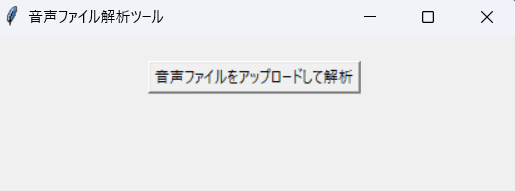
\includegraphics[width=\hsize]{fig/fig4-GUI_start.png}
    \caption{音声ファイル入力の画面}
    \label{fig:text}
\end{figure}

\begin{figure}[tb]
    \centering
    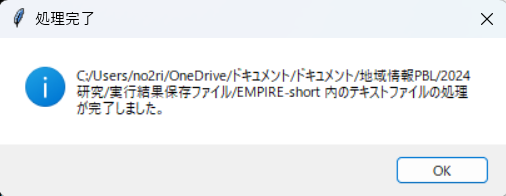
\includegraphics[width=\hsize]{fig/fig5-GUI_end.png}
    \caption{解析完了時の画面}
    \label{fig:text}
\end{figure}

\section{検証}
本章では，構築したシステムの検証手順とその結果を記述する．

\subsection{「Slow Motion Dream」での検証}
入力する楽曲は，Steven M Bryantの「Slow Motion Dream」の一部を使用する．
この楽曲は，インターネット上で公開されているフリーミュージックである．

この楽曲はelectric guitar，drum，vocalで構成されている．

\subsection{「EMPIRE」での検証}
入力する楽曲はsnowmanの「EMPIRE」冒頭1分19秒を使用する．

この楽曲はモーツァルト作曲「交響曲第25番ト短調K.183」の第一楽章をサンプリングした楽曲であり，イントロと呼ばれる冒頭部分ではサンプリング元楽曲の冒頭部分である第一楽章の第一主題が流れ，その後ロック調のメロディで構成される．
また，間奏部分においてもサンプリング元楽曲が流れており，classicとjazzの要素が時間水位に伴い混在する楽曲となっている．
このように本楽曲は時間遷移に伴いジャンルが変化しているため，システムの検証に適していると考えた．

検証結果のヒストグラムを\figref{fig:EMPIRE_short_jazz}，\figref{fig:IMPIRE_short_rock}，\figref{fig:EMPIRE_short_classic}に示す．

\begin{figure}[tb]
    \centering
    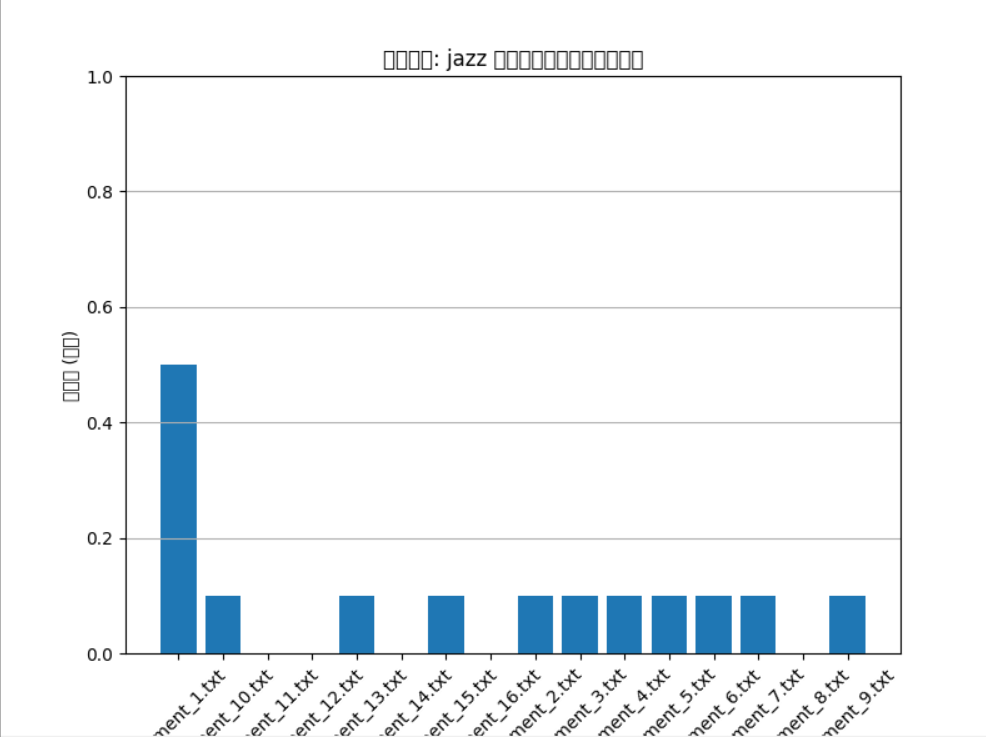
\includegraphics[width=\hsize]{fig/fig3-EMPIRE_short_jazz.png}
    \caption{EMPIREのjazzヒストグラム}
    \label{fig:text}
\end{figure}

\begin{figure}[tb]
    \centering
    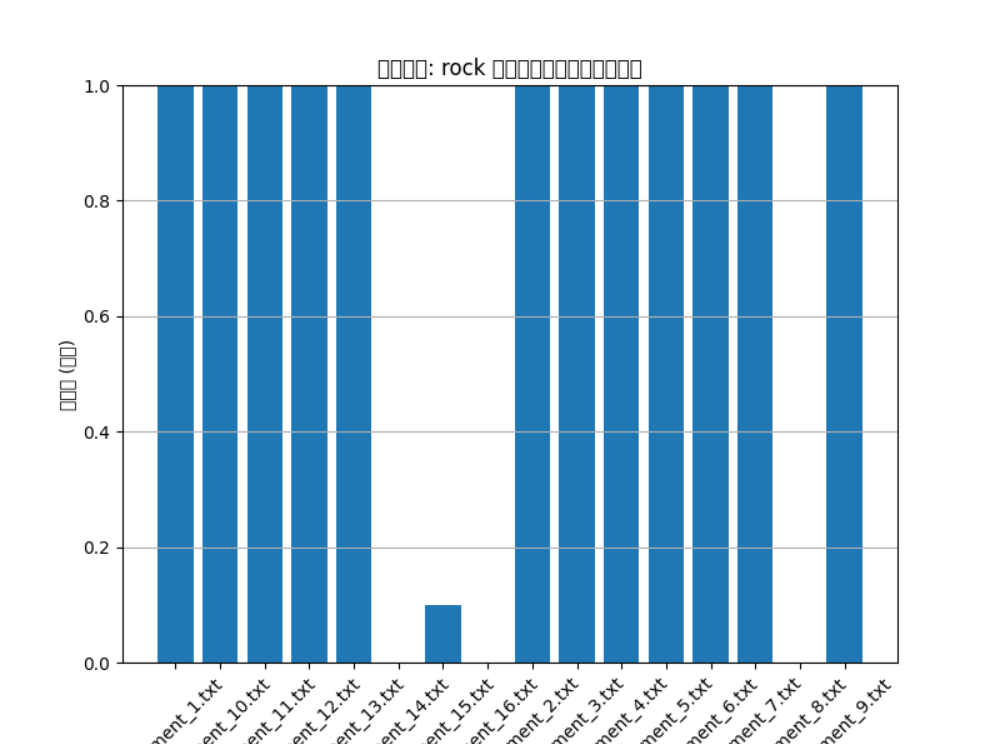
\includegraphics[width=\hsize]{fig/fig2-EMPIRE_short_rock.png}
    \caption{EMPIREのrickヒストグラム}
    \label{fig:text}
\end{figure}

\begin{figure}[tb]
    \centering
    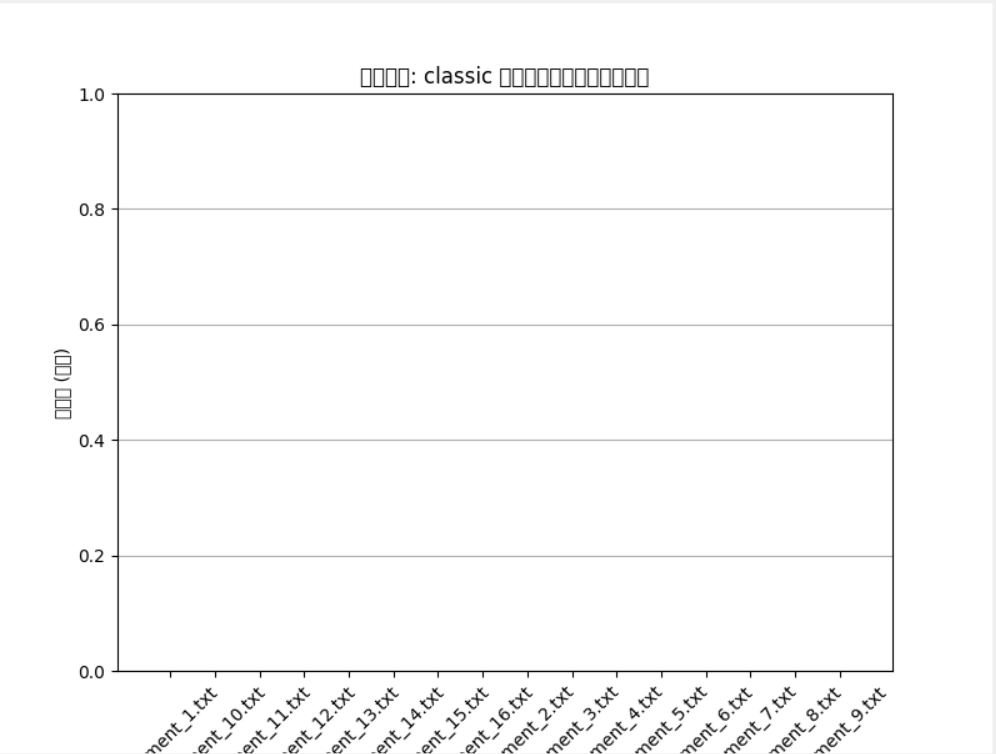
\includegraphics[width=\hsize]{fig/fig1-EMPIRE_short_classic.png}
    \caption{EMPIREのclassicヒストグラム}
    \label{fig:text}
\end{figure}

対象楽曲の冒頭5秒間の楽器構成はviolin，viola，cello，contrabass，oboe，faggot，corn，horn，vocal，drumである．
そのため，classicの一致度が高くなることが考えられた．

しかし，実装結果はclassicの一致度が0となっている．
データベースのClassic楽曲にはvocalが使用されている楽曲がないため，このような結果が出ていると考えられる．

また，冒頭5秒間のセグメントにて取得した楽器構成リストは，['vocal']のみである．
対象楽曲で試用されている楽器数が多いため，テキスト生成の際に正確に楽器を抽出できなかったものと考えられる．

\section{今後の課題}
\section{おわりに}

\begin{acknowledgment}
    %本稿の執筆にあたり，参考文献に挙げた方々のWebサイト，スライド，各種資料を大いに参考にさせていただいた．
    書くならお好きに
\end{acknowledgment}

